\documentclass{article}
\usepackage{graphicx}
\usepackage[spanish]{babel}
\begin{document}
	\begin{titlepage}
		\centering
		\vfill
		\fbox{\Huge{Sexta práctica}} \\
		\vfill
		\large{\textsc{Hugo Tonatiuh Carrillo Bonilla}}\\
		\vfill
		320026379
		\vfill
		\begin{center}
			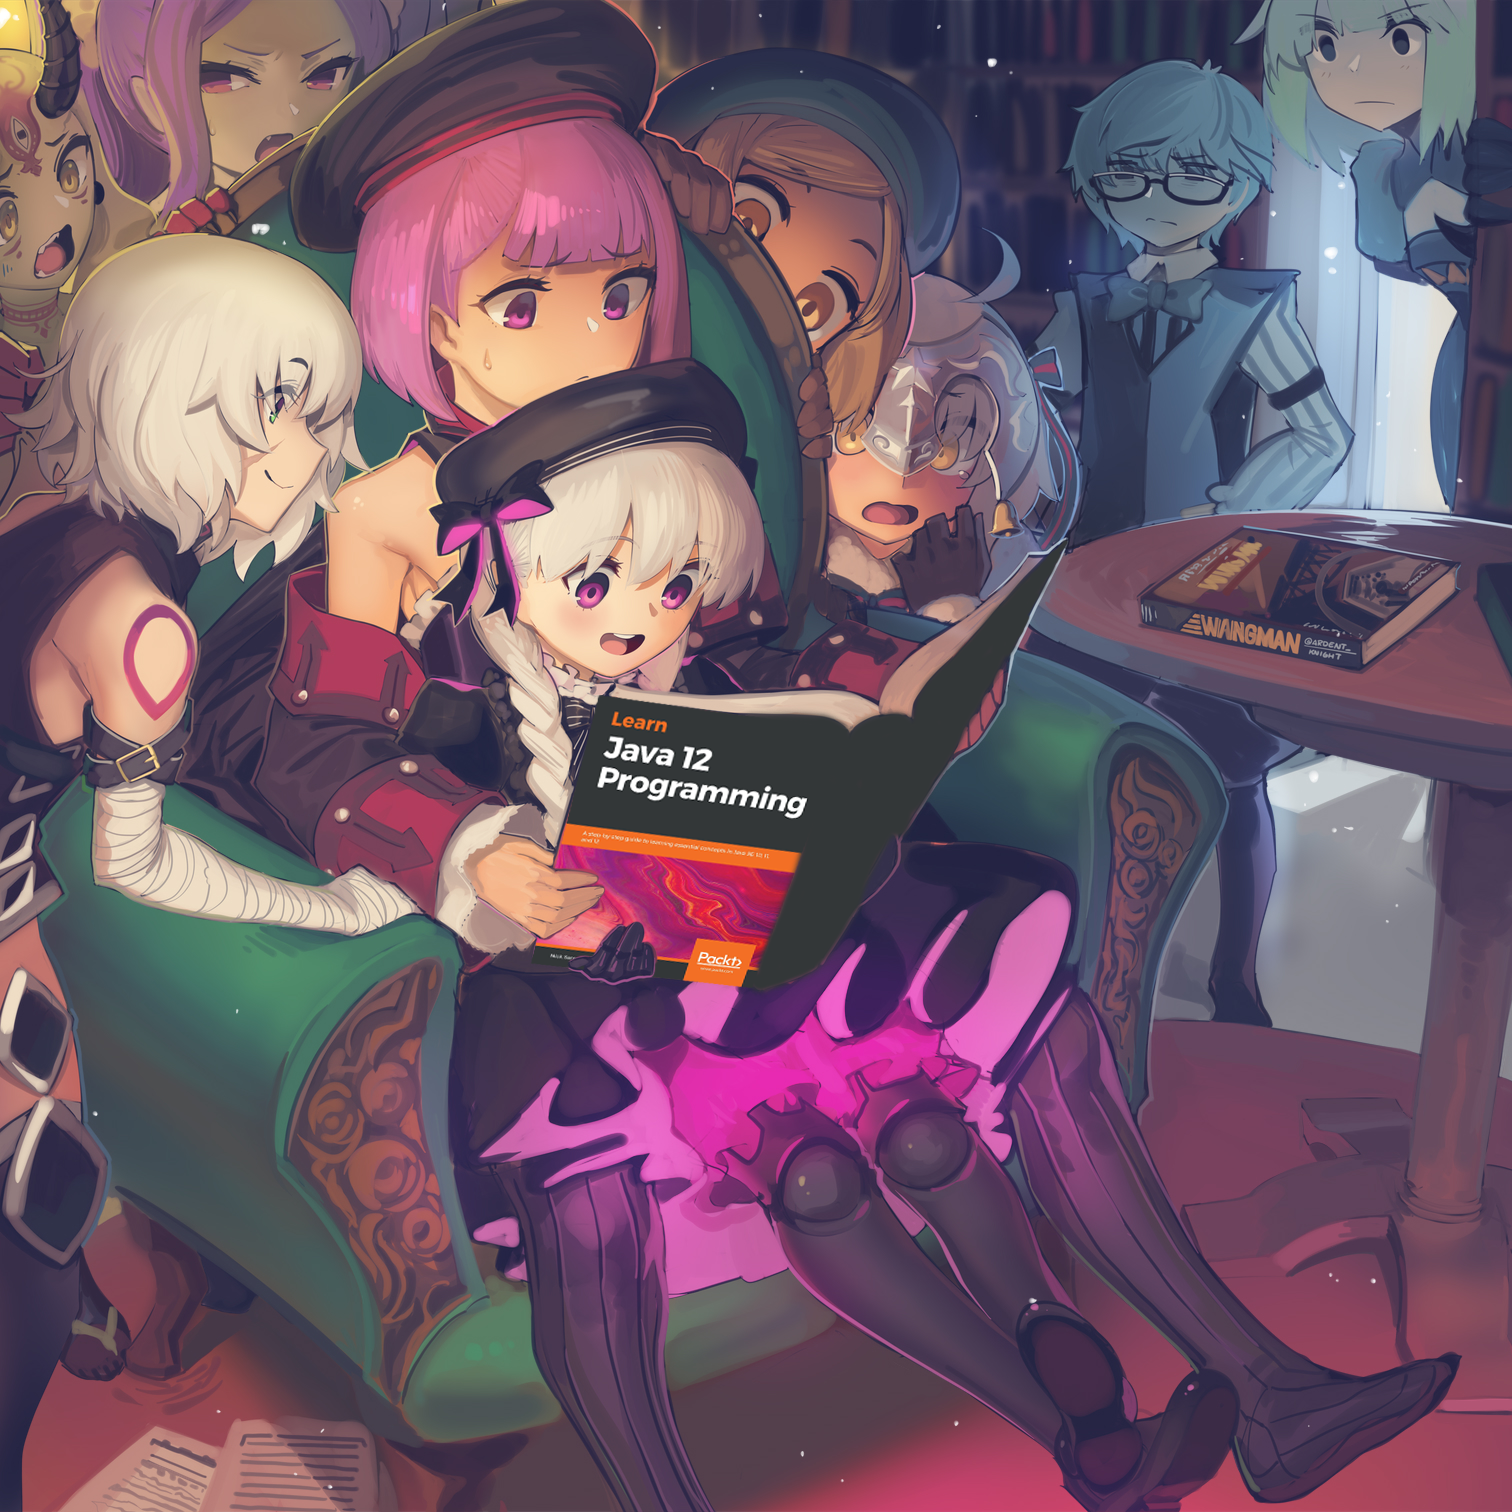
\includegraphics[width=\linewidth]{./images/Portada.png}
		\end{center}
		\vfill
	\end{titlepage}
	\section*{Parte 1: Conociendo Scanner}
		\section*{Actividad 1.1 - Dardos a la medida}
			\begin{itemize}
				\item \texttt{hasNexInt} verifica si el siguiente token se puede interpretar como \texttt{int}, regresa un boolean. \texttt{nextInt}
					fuerza a Scanner a interpretar el siguiente token como un entero, por esto regresa un \texttt{int}.
				\item El programa falla al momento de ejecución, si no anticipamos ese error.
				\item Usamos el \texttt{boolean} de \texttt{hasNexInt} como la condición para un \texttt{if} o \texttt{switch}.
			\end{itemize}
			Para resolver esta actividad, usé la estrategia en el punto pasado. Creé una variable booleana que funciona como centinela de un ciclo
			\texttt{while}, si \texttt{hasNexInt} regresa \texttt{true}, y el número que regresa es positivo, se cambia el valor del centinela y se sale
			del \texttt{while}. Hecho esto, se asigna el input a la variable de los dardos que se van a lanzar.
		\section*{Actividad 1.2 - Decimal a binario interactivo}
			El input se validó con la estrategia del ejercicio pasado. Para que el programa se repita hasta que la usuaria decida salir, se usa
			un \texttt{while} que reiteradamente escanea un input, valida que sea entero positivo y después realiza el algoritmo que vimos en la ayudantía
			teórica. La implementación de este algoritmo:
			\begin{enumerate}
				\item Usa variables auxiliares 
				\item Divide el número entre dos.
				\item Guarda el cociente.
				\item Guarda el residuo.
				\item Añade el residuo al principio de una cadena. 
				\item Este proceso se repite hasta que el cociente sea igual a 0.
			\end{enumerate}
			Hay un pequeño error de diseño que tengo que admitir: la condición del input se cambia manualmente en al final de cada iteración, aunque
			preferiría que esta se evaluara al inicio o que el mecanismo para que se ejecute la revisión del entero no dependa de una variable arbitraria.
	\section*{Parte 2: Bienvenidos a la Cabaña del Misterio}
		\section*{Actividad 2.1 - Programa final para la cabaña del misterio}
			Como esta actividad impone que todo esté dentro del método \texttt{main}, traté de modularizarlo lo más posible: la validación de datos y la
			ejecución del menú son relativamente independientes. La validación de datos usa \texttt{while} y \texttt{hasNexInt} como en las actividades
			pasadas. Así, se asignan las variables para calcular intereses. Cada bloque de código para las operaciones disponibles está dentro de un
			\texttt{case}, que se activa si el input de la usuaria. Es 1, 2, 3, 4 o 0. Según sea el caso. El cálculo del interés compuesto para la opción
			3 está escrita con un ciclo \texttt{for}. En cambio, el cálculo del interés compuesto para la comparación utiliza exponenciación.

			Todo  esto se ejecuta dentro de un ciclo \texttt{while} que es monitoreado por un centinela booleano. Este centinela booleano puede ser
			alterado manualmente, si el usuario elige la opción 0 (pésima práctica). También puede ser alterado si dos variables, que monitoreaan errores
			u operaciones efectivas, alcanzan un valor crítico.

			Para mi segunda ejecución, fui cliente preferente, pedí \$45988 prestados, los pagaría en 36 meses, con una tasa anual base del 15\%.
		\section*{Actividad 2.2 - Conclusión y retrospectiva}
			\underline{Sobre esta práctica:} yo la empecé el día en el que se subió, y sufrí mucho porque no entendía que el buffer de Scanner tiene que
			limpiarse después de leer un \texttt{nextInt()}. Después, no entendí que \texttt{hasNextInt} genera un booleano, y eso me permite verificar
			la entrada mediante condicionales. Irónicamente, eso solo lo entendí hasta que leí una respuesta en \textit{Stack Overflow} que también
			explicaba por qué se tenía que renovar el buffer de Scanner. Otro error común fue que mis ciclos centinela que iteraban el programa cargaban
			los valores de la iteración pasada, y los cálculos que devolvía el programa eran erróneos.
			\\
			\\
			\\
			\underline{A lo largo de este proyecto:} Ví cómo mi base de código crecía, añadiendo nuevas funcionalidades mientras se reutilizaba el código
			que ya había sido escrito. Se imponían nuevos requerimientos que complicaban considerablemente el desarrollo, encima, estos requerimientos
			habían sido especificados por el cliente desde el principio, solo que lo habíamos ignorado. Me sorprende mucho que, con estos dos
			impedimentos, nuestro proyecto haya llegado término, produciendo software funcional y completo. Sobre todo considerando que carecemos por
			completo de modularidad o de reusabilidad. Después de esto, siento muchísima más confianza en mis habilidades procedurales, y de detectar
			errores de lógica.
			\\
			\\
			\\
			\underline{Sobre el programa completo:} Estoy profundamente decepcionada y frustrada con él. Constantemente, me tardaba en encontrar errores
			de sintaxis, porque el error residía en una declaración o procedimiento anterior que era invocado después en ejecución. Además, debía de
			explicar lo que sucedía en la ejecución de TODO el programa, en lugar de lo que sucedía dentro de un solo módulo, para poder explicar el
			origen de mis errores de lógica. El código es repetitivo, tedioso e inmantenible.
\end{document}
